\chapter{Finite Automaton as Regular Language Recognizers}
	\section{Preliminar definitions}
	You should know what a FSA is. In particular, you should know well DFSAs\\
	A Finite State Machine (or finite state automaton) is composed of a set of states, a transiction function (that determines the change of state at a certain input) a 
	set of termination states, and an input alphabet.\\
	\textbf{\underline{A DFSA is expressive as an unilinear grammar}} (so like a regular expression).\\

	What we want to do is to use FSA as parsers to determine if a specific string belongs to a language.
	\begin{definition}[Accepted / Regognized string]
		a string x is accepted (recognized) iff the automaton,
		starting from initial configuration with x $\dashv$ as input
		performs a computation and reaches a final configuration
	\end{definition}

	From FSA theory we can state that a computation ends when the automaton:
	\begin{itemize}
		\item raches a final configuration ($\Rightarrow$ string is accepted), or
		\item no move can be executed ($\Rightarrow$ string not accepted)
	\end{itemize}

	\begin{definition}[Equivalent automata]
		Two automata accepting the same language are called equivalent.
	\end{definition}

	\begin{definition}[String recognized]\label{def:recstr}
		A string $x$ is recognized (or accepted) by automaton $M$ if and only if when scanning $x$, $M$ goes from the initial to the final state.
	\end{definition}

	\begin{definition}[Language recognized]
		A Language is recognized by automaton $M$ if all its strings are recognized\footnote{See definition \ref{def:recstr}.}
	\end{definition}

	\begin{definition}[Finite-state recognizable]
		The family of languages accepted by finite state automata is called finite-state recognizable.
	\end{definition}

	\begin{definition}[Completed FSA]
		The transition function can always be made complete by means of an \textbf{error state} $q_{err}$:
		\begin{align*}
			\forall \mbox{ state } q\in Q \mbox{ and } \forall \mbox{ symbol } a\in\Sigma\\
			\mbox{ if } \delta\left(q,a\right) \mbox{ is undefined }\\
			\mbox{ and } \forall \mbox{ symbol } a\in \Sigma \mbox{ let } \delta \left(q_{err},a\right)=q_{err}
		\end{align*}
	\end{definition}
	\section{Clean automaton}\label{sect:cleanautom}
		A state can be useful or useless. A state is useful if it is reachable from an initiale state and a final state can be reached from it (condition of accessibility and post-accessibility). Otherwise it's useless.
		\begin{property}
			For every finite automaton there exists an equivalent clean automaton.
		\end{property}
		To clean an automaton it can be easily flooded starting from the initial state then starting from the final state(s); all states not flooded at the end are useless.
	
		\begin{definition}[Undistinguishable states]\label{def:undiststates}
			Two state are undistinguishable if applying the same input to the both reach a final state or both do not.
		\end{definition}
		 This relation looks like it does not provide a tool to effectively 
		distinguish two state, but it's a RECURSIVE DEFINITION:
		\begin{itemize}
			\item The sink state (or error state) is distinguishable from all other state;
			\item If a state is final is distinguishable from every other non final state;
			\item Two states are distinguishable \textbf{if their next state is distinguishable}.
		\end{itemize}
		\textbf{Note}: State $p$ and state $q$ are different (and distinguishable) if the set of labels of the arcs outgoing from $p$ and $q$ are different.\\

		\emph{Indistinguishability} is a binary \textbf{relation}; it is \textbf{reflexive}, \textbf{symmetric}, and \textbf{transitive} hence it is an \textbf{equivalence relation}.

		\subsection{Minimization}
			States of the minimal automaton $M'$: the \emph{equivalence classes of the indistinguishability relation} transition function, arcs among equivalence classes:
			$$[\ldots,p_r, \ldots] \overset{b}{\longrightarrow} [\ldots, q_s, \ldots] \Rightarrow [p_r] \overset{b}{\longrightarrow} [q_s]$$
			\begin{property}[Minimal automaton - uniqueness property]
				For every finite state language, the finite recognizer is minimal w.r.t. the number of states exists and is unique (apart from a renaming of states)
			\end{property}
			This property enables to represent a whole class of equivalent automata with a single one, that moreover is \emph{minimal}.\\
			An algorithm to reduce automaton to their minimal equivalent is based on the equivalence relation between states called \emph{distinguishablity}.	
	\section{Nondeterministic Automata}
		As a unilinear grammar rule can contain multiple alternatives for the same nonterminal, a FSA can have multiple states associated to a input symbol.
		Moreover, an automaton could also have spontaneous moves, so arcs that are not associated with any kind of input, besides the empty string.
		
		%//TODO re-write definition of NFSA
		If one or both these two kinds of situation happen to be in a FSA it's called nondeterministic, due to the nondeterminism of the output (same input can lead to different output).\\
		There are a few motivations to add nondeterminism to an automaton:
		\begin{itemize}
			\item Concision: a nondeterministic automaton is often smaller than his deterministic counterpart, rendering the former more readable
			\item Mapping to grammars: as said, multiple alternative rules are more easily mapped on a NFSA than on a FSA
			\item Language reversing: when reversing an automaton (so changing arrows direction and initial/final states) nondeterminism often pops out
			\item ND recognizers: NFSA can be used to draft out a recognizer automaton
		\end{itemize}
		\subsection{Elimination of nondeterminism}
			The final implementation of a recognizer automaton must be deterministic (for now).
			\begin{theorem}\label{th:NFSA_TO_DFSA}
				Every nondeterministic automaton can be transformed in a deterministic equivalent one.
			\end{theorem}
			The theorem~\ref{th:NFSA_TO_DFSA} lets to the definition of:
			\begin{corollary}
				Every unilinear grammar\footnote{See section: \ref{sec:uni_linear_grammars}}  admits a equivalent nonambiguous one.
			\end{corollary}
			We focus on removing spontaneous moves to do we introduce:
			\paragraph{Backward propagation method}
				\begin{enumerate}
					\item Compute the transitive closure of $\epsilon$ moves: if three states are connected sequentially by spontaneous moves, add all the $\epsilon$ moves that shows all the $\epsilon$ paths.
					\item Backward propagation of the scanning moves over the epsilon moves: if a path contains a normal scan move AND a spontaneous move, then connect the first and last states of that path with a scan move with the element scanned.
					\item Add all the states that spontaneously arrive to the final state to the final states set.
					\item Delete all $\epsilon$ moves left.
				\end{enumerate}
				
			\begin{definition}[Ambiguity]
				As for the grammars, an automaton is ambiguous if it accepts a string with two different computations. 
			\end{definition}
	
	\section{Automaton to regexp - Brzozowski McCluskey method}
		The Brzozowski McCluskey method (BMC) method allows to generate a regular expression from an automaton that produces the same language.\\
		Assumptions:
		\begin{itemize}
			\item unique initial state
			\item initial state has no incoming arcs
			\item unique final state
			\item final state has no outgoing arcs
		\end{itemize}
		%The algorithm is quite simple: at every step, an internal node is removed and substitued by a set of arcs labeled as regular expressions (the additional arcs must not modify the automaton behaviour, obiously. They should compensate with the regexp the introduce the lack of the removed state). The algorithm terminates when only initial state and final state are left, so one only arc with a single regexp, equivalent to the whole automaton.\\
		Before seeing the algorithm, we need to consider the initial state $i$, the final state $t$ and define internal states.
		\begin{definition}[Internal states]
			Every state other than initial state $i$ and final state $t$ is called \textbf{internal}.
		\end{definition}
		\begin{algorithm}[Brzozowski McCluskey (BMC) method]
			\begin{itemize}
				\item[]
				\item If initial state $i$ has arcs incoming, add a new initial state with a spontaneous move ($\varepsilon$ move) to the original initial state. Do the
				similar thing to the final state $t$ if it has others outgoing arcs (note that now the ex-initial node and the ex-final node have become \emph{internal}).
				\item Until there are internal nodes:
				\begin{itemize}
					\item Consider an internal node to be removed;
					\item Construct an equivalent automaton (called \emph{generalized}), which will be more flexible because it allows the arc labels to be not just
					terminal characters, but also regular languages (labels can be r.e.).
				\end{itemize}
			\end{itemize}
			Once every node has been eliminated, we are left with only two nodes ($i$,$t$) and one arc. At this point, the label of the arc $i\longrightarrow t$ is the 
			r.e. of the language.
		\end{algorithm}
		Notes for nerdier people: this methods is similar (if not the same) to the one used to pass from an unilinear grammar to a regexp making use of "linear language equations".
		\begin{figure}[htp]
			\centering
			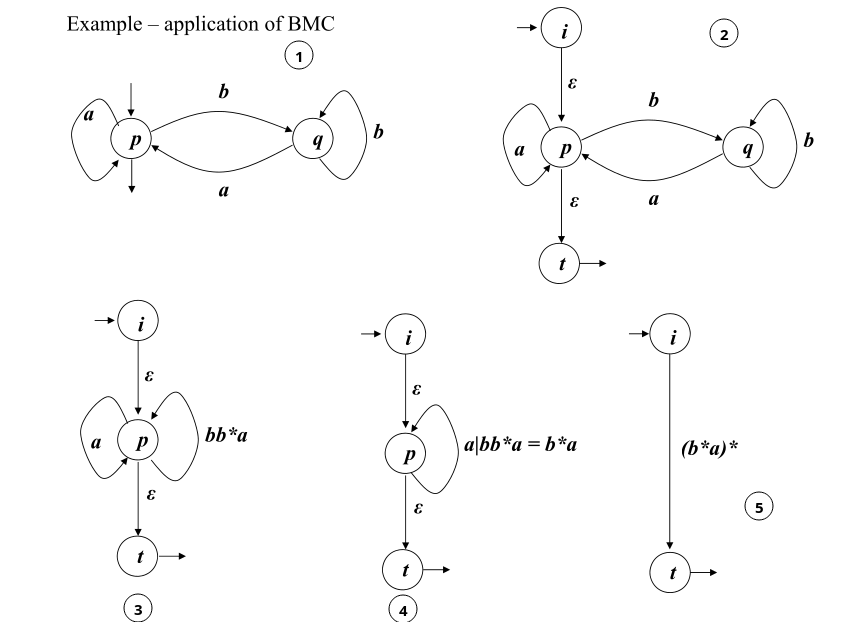
\includegraphics[width = \textwidth]{./images/BMCMethod.png}
		\end{figure}
	
	\section{Regexp to non deterministic recognizer - the Thompson Structural Method}
		Thompson's method analyzes a regexp by simple parts and generates the components associated to them. It then interconnects the components to build the whole automaton. A parallel is drawn between the operators in a regexp and the finite state components they generate.
		\begin{itemize}
			\item An \textbf{atomic expression} is just translated as an arc between two states. The empty string is considered an atomic expression.
			\item \textbf{Concatenation} is expressed as a spontaneous move that connects two states, a single epsilon arc.
			\item On the other hand, \textbf{alternatives} are parallel blocks of states; all blocks connected to a single entry state and a single exit state through epsilon moves.
			\empty The \textbf{star closure} instead is built as a recursive block of components, encapsulated in a initial and final state. The extreme steates are connected by a epsilon move.
		\end{itemize}
		Example:
		\begin{figure}[H]
			\begin{center}
			    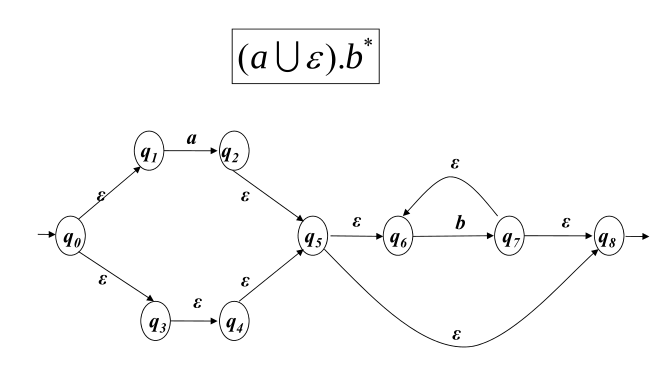
\includegraphics[width = \textwidth]{./images/ThompsonMethod.png}
			\end{center}
		\end{figure}
		
	\section{Regexp to deterministic automaton - Berry Sethi Method}
		\subsection{Theorical fundament: local languages and local automata}
		%//TODO check the theory of local languages -> still missing how to recognize if s.thing is local and local automaton (definitions useful for practical exercises)
			In order to fully understand the Berry Sethi method (ahaha) we must introduce the family of local languages.
			\begin{definition}[Local sets]
				For a language $L$ over an alphabet $\Sigma$, the set of \textbf{initials} is:
				$$Ini(L)=\lbrace a\in\Sigma\vert a\Sigma^*\cap L\neq\emptyset\rbrace$$
				i.e., the starting characters of the sentences. The set of \textbf{finals} is:
				$$Fin(L)=\lbrace a\in\Sigma\vert \Sigma^* a\cap L\neq\emptyset\rbrace$$
				i.e., the ending characters of the sentences. The set of \textbf{digrams} (factors) is:
				$$Dig(L)=\lbrace x\in\Sigma^2\vert\Sigma^*\times\Sigma^*\cap L\neq\emptyset\rbrace$$
				i.e., the substrings of length two present in the sentences. The three sets abve are called \textbf{local}.
				The complementary of digrams are:
				$$\overline{Dig(L)}=\Sigma^2/Dig(L)$$
			\end{definition}

			\begin{definition}[Local language]
				A language $L$ is called local (or locally testable) if it satisfies the following identity:
				$$L/\lbrace\varepsilon\rbrace =\lbrace x\vert Ini(x)\in Ini(L)\wedge Fin(x)\in Fin(L)\wedge Dig(x)\subseteq Dig(L)\rbrace$$
				In other words, the non empty phrases of language $L$ are defined precisely by sets $Ini$, $Fin$, and $Dig$.
			\end{definition}


			The complement of the diagram set is also an important set to consider.\\
			\begin{corollary}
				A local language is called so \emph{iff} the non empty sentences of that language are exactly definable through combinations of the three Ini, Fin and Dig sets.
			\end{corollary}
			\begin{corollary}
				Local language must include \emph{all and only} the local sentences, generated by combining Ini, Dig e Fin.
			\end{corollary}

			In general, it's possible for a language to define a Dig set of diagrams that (for example) can be generated only in a certain order.
			So not all possible combination of diagrams can be obtained.\\
			So, with the above example, we have demonstrated that type of language is not a local language.
			\begin{definition}[local automaton]
				A deterministic automaton $(Q, \Sigma, \delta, q_0 , F)$ is called local if it satisfies the condition:
				$$\forall a \in \Sigma \quad \lvert \{ \delta(q, a) : q \in Q \} \rvert \leq 1$$
				which forbids that two identically labeled arcs enter distinct states.
			\end{definition}

			\begin{property}
				A word can be established as member of a given local language by watching only two characters of it. 
			\end{property}
			\subsubsection{Local language recognizer}
				Building a recognizer for a local language is extremely simple: due to the "window of fixed length" to recognize a word, a 4 state automaton is enough.
				\begin{enumerate}
					\item Verify that the initial char is in Ini,
					\item Verify that all the couples are in Dig,
					\item accept if last char is in Fin.
				\end{enumerate}
				This algorithm can be fully carried out by a finite automaton. This automaton should be built this way:
				\begin{itemize}
					\item a unique initial state q\textsubscript{0} that's also final if $\epsilon$ is in the language;
					\item a set of final states F = Fin;
					\item a transiction function: 
						\begin{equation}
							\delta =
							\begin{cases}
							  \forall a \in \text{Ini} \text{  } \delta(q\textsubscript{0}, a) = a \\
							  \forall x y \in \text{Dig} \text{   } \delta(x y) = y
							\end{cases}
					  	\end{equation}
				\end{itemize}
				An automaton is said \emph{local} if it satisfies the condition 
				\begin{equation}
					\forall a \in \text{Alphabet, } q \in \text{States }  \vert \{ \delta(a, q) \} \vert <= 1 
				\end{equation} 
				That translates in "two identically labeled arcs cannot enter distinc states".\\
				A \emph{normal local automaton} satisfies also the two following properties:
				\begin{itemize}
					\item The state set is exactly the values in the alphabet plus the initial state;
					\item All and only the arcs labeled \emph{a} enters state \emph{a}. This implies no arcs enter the inital state.
				\end{itemize}
				
			\subsubsection{Equivalence between local automaton and local language}
				For any language L the three conditions
				\begin{itemize}
					\item L is local
					\item L is recognized by a local automaton
					\item L is recognized by a normal local automaton
				\end{itemize}
		
		\subsection{The Berry Sethi Algorithm}
			The Berry Sethi algorithm exploits the properties of local languages to obtain a deterministic recognizer for any regular expression.\\
			To do so, we must introduce a new set of terminals (to the Ini, Dig and Fin) that is the Fol(lower). It is defined as the set of characters that can appear right next to one, given. It carries the same information of the Dig set, and it's defined from that:
			\begin{equation}
				\text{Fol}(a) = \{ b \vert ab \in \text{Dig} \}
			\end{equation}
			If no followers exists for a certain symbol, the $\dashv$ symbol signals it. So, id \emph{reg} is our regular expression, then "\emph{reg}$\prime \dashv$" is the numbered version of \emph{reg} followed by the terminator. "Numbered" just means that every character in the regexp has a unique numeric identifier.\\
			The algorithm is composed of three main parts:
			\begin{enumerate}
				\item Initial state definition: the initial state is marked as the Ini set of the regexp analyzed (Ini(\emph{reg}$\prime \dashv$)).
				\item Every distinct element in the Ini state will label an outgoing arc from the initial state. REMEMBER: even though the regexp is numbered, arcs and states uses the nonnumbered version of the characters. 
				\item Every state is named (labeled) as the set of followers of the read character (the one on the followed arc). 
				\item The steps 2 and 3 are repeated until no more states can be generated. The final states are the ones that have in the followers set $\dashv$.
			\end{enumerate}
			
			\subsubsection{Berry Sethi algorithm as automata determinizing process}
				The BS algorithm can be also used to convert a nondeterministic machine into a deterministic one. It's very easy to do so: it is enough to number all the characters on the non-spontaneous moves of the starting automaton, compute the obtained Ini, Fol and Fin sets from the language obtained, then applying BS algorithm to the language obtained. The result is a deterministica automaton that recognizes the same language as the starter one. 
			
	\section{Recognizers for Complement and Intersection}
		As regular languages can be complemented and intersected, so can their recognizer automata be transformed to match such operations.\\
		Algorithm to complement a DFSA regular recognizer:
		\begin{enumerate}
			\item Add the sink state
			\item Connect all the states to the sink state, wheter a state cannot read a character (for example, on the alphabet {a, b}, if state q cannot cannot read "a" an arc q $\rightarrow$ sink state is added, labeled "a")
			\item Reverse the final with the initial state
		\end{enumerate}
		
		Due to the De Morgan identity L $\cap$ R = !(!L $\cup$ !R), where "!" is the complement, it's sufficient to know an algorithm for complementing the recognizer to also build one for the interception. 